\documentclass[cn]{elegantbook}
\usepackage[square,numbers,sort&compress]{natbib}
\newcommand{\upcite}[1]{\textsuperscript{\textsuperscript{\cite{#1}}}}
\usepackage{diagbox}
\usepackage{algorithm}
\usepackage{algorithmicx}
\usepackage{algpseudocode}
\renewcommand{\algorithmicrequire}{\textbf{输入:}}
\renewcommand{\algorithmicensure}{\textbf{输出:}}

\tikzstyle{startstop} = [rectangle, rounded corners, minimum width = 2cm, minimum height=1cm,text centered, draw = black, fill = red!40]
\tikzstyle{arrow} = [->,>=stealth]

% title info
\title{模式识别作业5}
\subtitle{贝叶斯分类}
% bio info
\author{罗雁天}
\institute{清华大学电子系}
\version{2018310742}
\date{\today}
\logo{logo.png}
\cover{cover.jpg}

\begin{document}

\maketitle
\tableofcontents
\mainmatter
\hypersetup{pageanchor=true}
% add preface chapter here if needed
\chapter{问题描述}
设有符合正太分布的两类样本,并且设$P(\omega_1)=P(\omega_2)=0.5$.
\begin{equation}
\begin{aligned}
\omega_1&=\{(3,4),(3,8),(2,6),(4,6)\} \\
\omega_2&=\{(3,0),(3,-4),(1,-2),(5,-2)\}
\end{aligned}
\end{equation}
求解以下问题:
\begin{itemize}
	\item 求识别函数
	\item 求识别界面方程
	\item 绘制识别界面
\end{itemize}

\chapter{分类结果}
首先计算两个类的类均值:
\begin{equation}
M_1=[3,6], M_2=[3,-2]
\end{equation}

根据无偏估计的协方差矩阵计算方法:
\begin{equation}
\Sigma_i=\frac{1}{N-1}\left(\omega_i-M_i\right)^T\left(\omega_i-M_i\right)\quad i=1,2
\end{equation}

计算两个类的协方差矩阵:
\begin{equation}
\Sigma_1=\left[\begin{array}{cc}
0.6667 & 0\\
0 & 2.6667
\end{array}\right],\Sigma_2=\left[\begin{array}{cc}
2.6667 & 0 \\
0 & 2.6667
\end{array}\right]
\end{equation}

计算正态分布时贝叶斯判别准则所需要的参数如下:
\begin{equation}
\begin{aligned}
\mathbf{W}_1&=-\frac{1}{2}\Sigma_1^{-1}=\left[\begin{array}{cc}
-0.7500 & 0 \\
0 & -0.1875
\end{array}\right] \\
\mathbf{W}_2&=-\frac{1}{2}\Sigma_2^{-1}=\left[\begin{array}{cc}
-0.1875 & 0 \\
0 & -0.1875
\end{array}\right] \\
\mathbf{w}_1&=\Sigma_1^{-1}M_1=[4.50,2.25]^T; \\
\mathbf{w}_2&=\Sigma_2^{-1}M_2=[1.125,-0.75]^T; \\
w_{10}&=-\frac{1}{2}M_1^T\Sigma_1^{-1}M_1-\frac{1}{2}\ln |\Sigma_1|+\ln P(\omega_1)=-14.4808 \\
w_{20}&=-\frac{1}{2}M_2^T\Sigma_1^{-1}M_2-\frac{1}{2}\ln |\Sigma_2|+\ln P(\omega_2)=-4.1115
\end{aligned}
\end{equation}

对任意数据点$\mathbf{x}=[x_1,x_2]^T$,计算两类的识别函数如下:
\begin{equation}
\begin{aligned}
d_1(\mathbf{x})&=\mathbf{x}^T\mathbf{W}_1\mathbf{x}+\mathbf{w}_1^T\mathbf{x}+w_{10} \\
&=-0.75x^2-0.1875x_2^2+4.5x_1+2.25x_2-14.4808 \\
d_2(\mathbf{x})&=\mathbf{x}^T\mathbf{W}_2\mathbf{x}+\mathbf{w}_2^T\mathbf{x}+w_{20} \\
&=-0.1875x^2-0.1875x_2^2+1.125x_1-0.75x_2-4.1115
\end{aligned}
\end{equation}

则判别函数如下:
\begin{equation}
f(\mathbf{x})=\left\{\begin{array}{cc}
x\in\mbox{class1} & \mbox{if}\quad d_1(\mathbf{x})>d_2(\mathbf{x}) \\
x\in\mbox{class2} & else
\end{array}\right.
\end{equation}

计算识别界面如下:
\begin{equation}
d_1(\mathbf{x})=d_2(\mathbf{x})\Rightarrow -0.5625x_1^2+3.375x_1+3x_2-10.3693=0
\end{equation}

由此可以看出,分类界面在此种情况下是抛物线。

绘制出两个二维高斯分布的曲面如图\ref{gauss1}所示,识别界面如图\ref{res1}所示
\begin{figure}[!h]
	\centering
	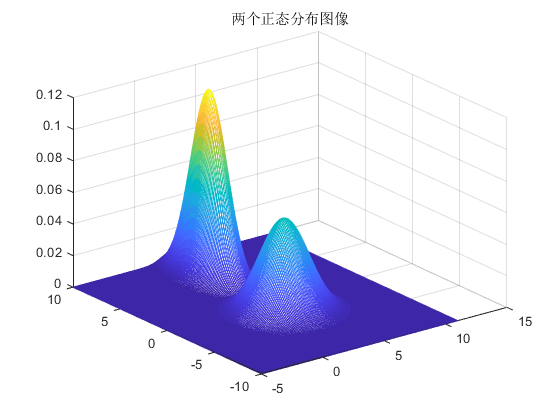
\includegraphics[width=0.7\linewidth]{gauss1}
	\caption{\label{gauss1}二维高斯分布密度函数曲面}
\end{figure}
\begin{figure}[!h]
	\centering
	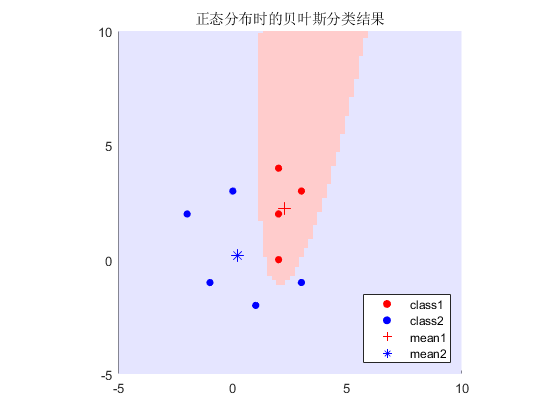
\includegraphics[width=0.7\linewidth]{res1}
	\caption{\label{res1}识别界面}
\end{figure}

\chapter{总结与反思}
根据课上的结论我们可以知道,对于二维数据的二分类问题,根据正态分布时贝叶斯判别准则我们可以知道,分类界面主要有三种情况:
\begin{itemize}
	\item 当$\Sigma_i=\sigma^2I,i=1,2$时,分类界面是两类均值连线的中垂线;
	\item 当$\Sigma_1=\Sigma_2$时,分类界面是过两类均值连线中点的直线(一般不垂直);
	\item 当$\Sigma_1\ne\Sigma_2$时,分类界面是二次曲线(圆、椭圆、双曲线、抛物线等)。
\end{itemize}

以下,我们通过修改数据分别模拟以上几种情况的分类界面。
\section{$\Sigma_1=\Sigma_2=\sigma^2I$}
修改数据为:
\begin{equation}
\begin{aligned}
\omega_1&=\{(3,4),(3,8),(1,6),(5,6)\} \\
\omega_2&=\{(1,0),(1,-4),(-1,-2),(3,-2)\}
\end{aligned}
\end{equation}
绘制出两个二维高斯分布的曲面如图\ref{gauss2}所示,识别界面如图\ref{res2}所示,从中可以看出,分类界面是两类均值连线的中垂线;
\begin{figure}[!h]
	\centering
	\begin{minipage}{0.48\linewidth}
		\centering
		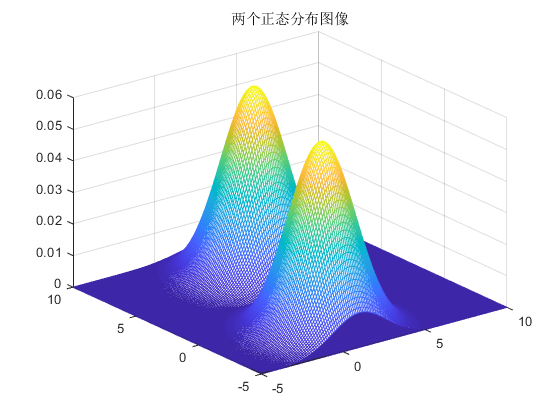
\includegraphics[width=\linewidth]{gauss2}
		\caption{\label{gauss2}二维高斯分布密度函数曲面}
	\end{minipage}
	\begin{minipage}{0.48\linewidth}
		\centering
		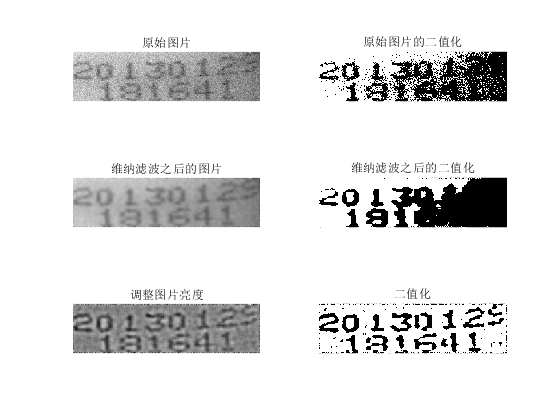
\includegraphics[width=\linewidth]{res2}
		\caption{\label{res2}识别界面}
	\end{minipage}
\end{figure}

\section{$\Sigma_1=\Sigma_2\ne\sigma^2I$}
修改数据为:
\begin{equation}
\begin{aligned}
\omega_1&=\{(3,4),(3,8),(2,6),(4,6)\} \\
\omega_2&=\{(1,0),(1,-4),(0,-2),(2,-2)\}
\end{aligned}
\end{equation}
绘制出两个二维高斯分布的曲面如图\ref{gauss3}所示,识别界面如图\ref{res3}所示,从中可以看出,分类界面是过两类均值连线中点的直线(一般不垂直);
\begin{figure}[!h]
	\centering
	\begin{minipage}{0.48\linewidth}
		\centering
		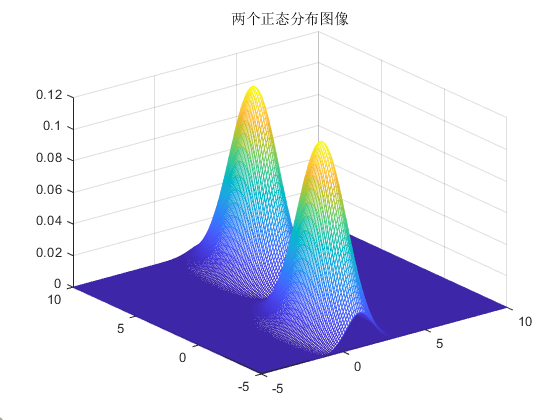
\includegraphics[width=\linewidth]{gauss3}
		\caption{\label{gauss3}二维高斯分布密度函数曲面}
	\end{minipage}
	\begin{minipage}{0.48\linewidth}
		\centering
		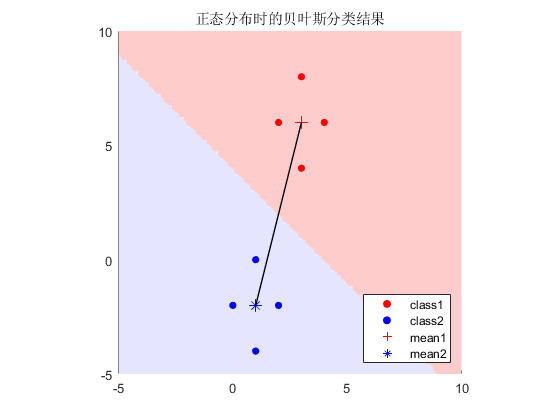
\includegraphics[width=\linewidth]{res3}
		\caption{\label{res3}识别界面}
	\end{minipage}
\end{figure}

\section{$\Sigma_1\ne\Sigma_2$}
原问题即是分类界面为抛物线的情况,在此不再考虑。
\subsection{分类界面为圆}
修改数据为:
\begin{equation}
\begin{aligned}
\omega_1&=\{(3,5),(3,7),(2,6),(4,6)\} \\
\omega_2&=\{(3,0),(3,-4),(1,-2),(5,-2)\}
\end{aligned}
\end{equation}
绘制出两个二维高斯分布的曲面如图\ref{gauss4}所示,识别界面如图\ref{res4}所示,从中可以看出,分类界面是圆;
\begin{figure}[!h]
	\centering
	\begin{minipage}{0.48\linewidth}
		\centering
		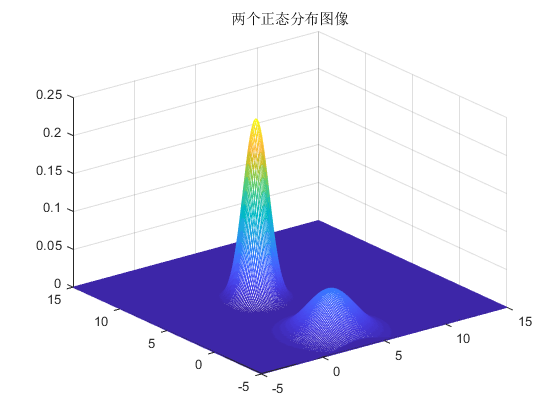
\includegraphics[width=\linewidth]{gauss4}
		\caption{\label{gauss4}二维高斯分布密度函数曲面}
	\end{minipage}
	\begin{minipage}{0.48\linewidth}
		\centering
		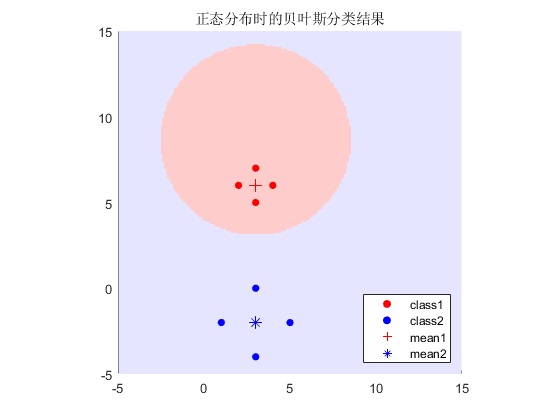
\includegraphics[width=\linewidth]{res4}
		\caption{\label{res4}识别界面}
	\end{minipage}
\end{figure}

\subsection{分类界面为椭圆}
修改数据为:
\begin{equation}
\begin{aligned}
\omega_1&=\{(3,4),(3,8),(2,6),(4,6)\} \\
\omega_2&=\{(3,1),(3,-5),(1,-2),(5,-2)\}
\end{aligned}
\end{equation}
绘制出两个二维高斯分布的曲面如图\ref{gauss5}所示,识别界面如图\ref{res5}所示,从中可以看出,分类界面是椭圆;
\begin{figure}[!h]
	\centering
	\begin{minipage}{0.48\linewidth}
		\centering
		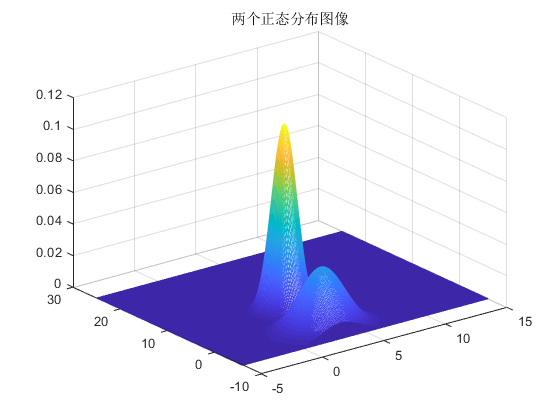
\includegraphics[width=\linewidth]{gauss5}
		\caption{\label{gauss5}二维高斯分布密度函数曲面}
	\end{minipage}
	\begin{minipage}{0.48\linewidth}
		\centering
		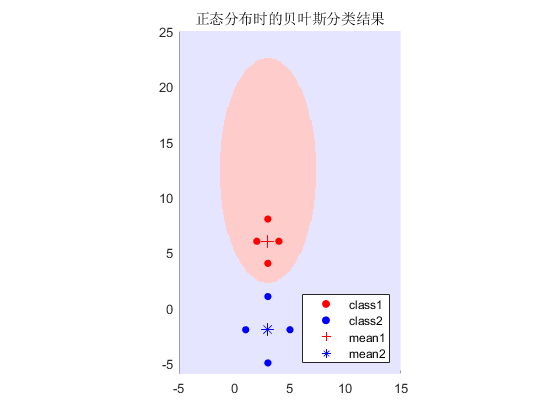
\includegraphics[width=\linewidth]{res5}
		\caption{\label{res5}识别界面}
	\end{minipage}
\end{figure}

\subsection{分类界面为双曲线}
修改数据为:
\begin{equation}
\begin{aligned}
\omega_1&=\{(3,4),(3,8),(2,6),(4,6)\} \\
\omega_2&=\{(3,-1),(3,-3),(1,-2),(5,-2)\}
\end{aligned}
\end{equation}
绘制出两个二维高斯分布的曲面如图\ref{gauss6}所示,识别界面如图\ref{res6}所示,从中可以看出,分类界面是双曲线;
\begin{figure}[!h]
	\centering
	\begin{minipage}{0.48\linewidth}
		\centering
		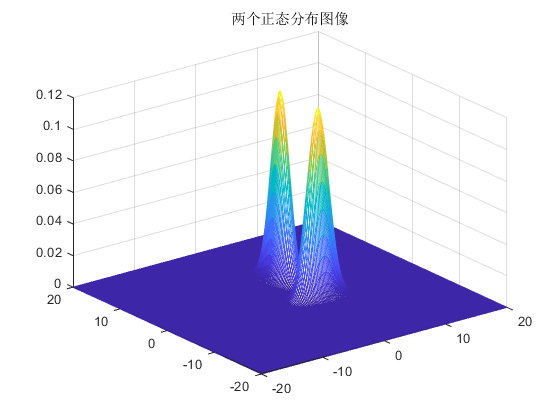
\includegraphics[width=\linewidth]{gauss6}
		\caption{\label{gauss6}二维高斯分布密度函数曲面}
	\end{minipage}
	\begin{minipage}{0.48\linewidth}
		\centering
		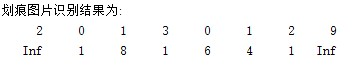
\includegraphics[width=\linewidth]{res6}
		\caption{\label{res6}识别界面}
	\end{minipage}
\end{figure}

\subsection{分类界面为退化的双曲线(双曲线的渐近线)}
修改数据为:
\begin{equation}
\begin{aligned}
\omega_1&=\{(3,4),(3,8),(2,6),(4,6)\} \\
\omega_2&=\{(4,3),(8,3),(6,2),(6,4)\}
\end{aligned}
\end{equation}
绘制出两个二维高斯分布的曲面如图\ref{gauss7}所示,识别界面如图\ref{res7}所示,从中可以看出,分类界面是两条直线;
\begin{figure}[!h]
	\centering
	\begin{minipage}{0.48\linewidth}
		\centering
		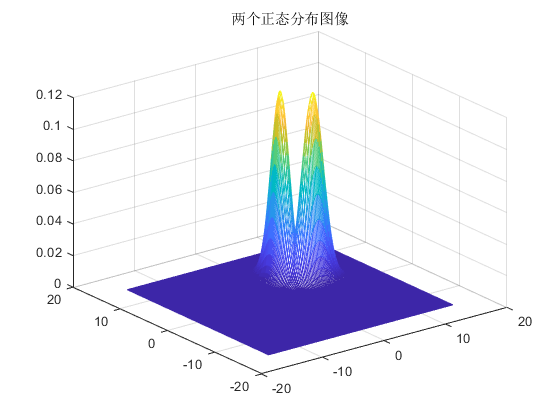
\includegraphics[width=\linewidth]{gauss7}
		\caption{\label{gauss7}二维高斯分布密度函数曲面}
	\end{minipage}
	\begin{minipage}{0.48\linewidth}
		\centering
		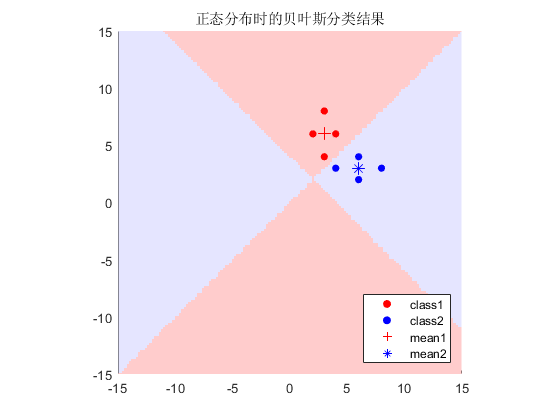
\includegraphics[width=\linewidth]{res7}
		\caption{\label{res7}识别界面}
	\end{minipage}
\end{figure}

\chapter{代码说明}
\noindent 本次实验使用Matlab语言编写,所有代码放置在“code/”文件夹下:
\begin{itemize}
	\item main.m: 以上讨论的各种情况执行的主函数,运行即可得到所有的分类界面图像以及二维正态密度函数的图像;
	\item Bayes\_Gauss.m: 使用高斯分布时的贝叶斯判别准则绘制分类界面的函数。
\end{itemize}

\end{document}